\documentclass[autodetect-engine,dvi=dvipdfmx,ja=standard,a4j]{bxjsarticle}

\usepackage[dvipdfmx]{graphicx}
\usepackage{amsmath}
\usepackage{caption}
\usepackage{fancyvrb}
\usepackage{fancybox}
\usepackage{hyperref}
\usepackage{color}
\usepackage[dvipsnames]{xcolor}
\usepackage{listings, jvlisting}
\usepackage{float}
\usepackage{wrapfig}
\usepackage{forest}
\usepackage{dirtree}
\usepackage{tcolorbox}

\setcounter{tocdepth}{3}

\definecolor{term-back}{HTML}{4A154C}
\definecolor{dircolor}{HTML}{1E90FF}

\newcommand{\cmd}[1]{\textcolor{yellow!70!white} {#1}}
\newcommand{\dirpath}[1]{\textcolor{Cerulean}{#1}}
\newcommand{\prompt}[1]{\texttt{\dirpath{#1}:\$ }}
\newcommand{\termtext}[2]{\Large{\prompt{#1}\texttt{#2}}}
\newtcolorbox{terminal}[1]{title={#1},fonttitle=\bfseries,colbacktitle=black!90!white,colframe=black,colback=term-back,coltext=white}

\lstset{
    language = C++,
    backgroundcolor={\color[gray]{.95}},
    breaklines=true,
    basicstyle = \ttfamily\scriptsize,
    keywordstyle={\bfseries \color[HTML]{0000CD}},
    commentstyle={\itshape \color[HTML]{17B233}},
    frame=single,
    framesep=5pt,
    numbers=left,
    numberstyle=\tiny,
    stepnumber=1,
    tabsize=4,
    captionpos=t,
    xleftmargin=2pt,
}

\title{\textbf{LinuxOSの基本とその操作}}
\author{作成:寺岡 久騎}

\date{最終更新日:\today}

\begin{document}
\maketitle

\begin{abstract}
    本資料ではロボット制御において,マイコンの範疇を超えてROSをはじめとした複雑なシステム及びプログラム
    をPC等のコンピュータ上で実行して使用する際によく利用されている\textbf{Linux系のOS}について,基本的な概要と
    その操作について簡単に説明する.また,解説において主に使用するOSは\textbf{Ubuntu 22.04 LTS}である.
    資料について不明点や内容に誤りがあれば作成者に連絡していただけるとありがたいです.あと一応この資料の
    利用は部内限定でお願いします.
\end{abstract}
\tableofcontents

\clearpage
\part*{まえがき}
こんにちは.資料作成者の寺岡です.ロボット研究会では制御班として主にプログラミングに関係する
作業を中心に活動しています.所属は工学部工学科情報・電気・数理データサイエンス系情報工学コースで,
この資料作成時点で3回生となっている身です.専攻が情報工学ということで資料の題材となっている
オペレーティングシステムやらプログラムやらコンピュータについて学んでいる訳ですが,ロボ研の資料としてこのあたりの専門の知識を
詰め込んでしまうと文章構成とかがややこしいことになるし,そもそも自分も全てを網羅しているわけではなく下手に頭にあることを全て書き連ねてしまうと
間違ったことを書いてしまうかもしれないので
細かい部分や背景の部分を結構省略して基礎的な部分・大事な事柄をフワッとした感じで
説明をしています.そのためこの資料は,記載している事柄や知識について完全にではなく「大体こんなイメージかなー」「こうすれば
こうゆうことが出来るんだー」くらいに捉えて,とりあえず多少実践にもっていけるくらいに理解してもらえることを目的にしています.
なので,見た目が少々小難しそうな資料ですがあまり身構えず気楽に読み進めてもらえたら幸いです.

この資料は{\LaTeX}\footnote{LaTeX:「ラテフ」と読む}っていう文書作成ツールを使って書いています.
主に理系で論文の執筆とかに使われていて,Wordの様に直接文章を書くのではなく,HTMLみたくソースコードに文章と図・写真の挿入や体裁の設定などを記述
して,これをビルドすることにより文書ファイルを出力してくれます.
Wordと比べて勝手に体裁を整えてくれたり,数式を記述するのが比較的楽だったりと良いところがあるんですが
細かいところまで見た目にこだわろうとするとかなり難しくてですね\dots
パッケージやらオプションやらをいじる必要があるので触りたての頃は書くのに結構苦労しました.
しかしながら情電数理の人は1年前期の工学基礎実験実習で講義の中でいきなりやらされるし,情報工学コースではプログラミング演習系の講義
の期末レポートは{\LaTeX}で書かされるので,僕自身それなりに触れているためか少し書くのに慣れてきたんですよ.すると思ったより便利に感じてきて,
今では「文書は全部{\LaTeX}で書けば良くね」みたいな思想というかノリになってしまいました.
なので今回勝手に{\LaTeX}で資料をゴリゴリ書いてみたわけですが,やはりまだ難しいと感じる部分はあるので
ミスってる箇所・分かりにくい箇所があると思いますので今後のためにもそのような部分を発見したらご指摘頂けるとありがたいです.
あと,文章中たまに自我が出てたりしますがあまり気にしないで下さい.
\clearpage

\part{事前知識} \label{foundation}

\section{この部の概要} 
この第\ref{foundation}部では
次のLinuxに関する解説をする上で読者に予め覚えておいてほしい
コンピュータやプログラム・OSに関する知識・用語の紹介と説明を行います.
以降の内容をちらっと見て何となく知っているなあと思ったら
読み飛ばしてもらって大丈夫です.

\section{コンピュータに関する用語} \label{sec:computer-knowledge}
この章ではコンピュータに関する基本的な用語について解説をします.
一言で「コンピュータ」というと,家電などの組み込み系に使われているマイコンとかまで
含んで指してしまい,内容が少し分かりづらくなってしまうので以降本書に登場する「コンピュータ」は自分たちが普段使用しているWindowsのPCとかMac
の様ないわゆる「パソコン」を意味していると解釈して下さい.\\

\textbf{用語一覧}
\begin{itemize}
    \item CPU
    \item ストレージ
    \item メモリ
    \item ファイル
    \item フォルダ・ディレクトリ
    \item ハードウェア
    \item ソフトウェア
    \item ビット・バイト
\end{itemize}

\subsection{CPU}
\textbf{CPU}は「Central processing Unit」の略称であり,
日本語では「中央演算処理装置」や「プロセッサ」などと呼ばれる装置のことである.

CPUは演算や様々なデータの処理を行う役割を果たす装置であり,
外部から与えられた命令を基に処理を実行する.人間でいうところの
頭脳にあたるものでありコンピュータの基本的な性能の高さはこのCPUの性能に比例する.

\subsection{ストレージ}
ストレージとはコンピュータで利用するデータ(ファイル)を保管する装置のことであり,
基本的にCPUの外部に取り付けられるため「外部記憶装置」「外部ディスク」などとも呼ばれる.
コンピュータの電源のON・OFFの状態に関わらずデータを保存できる.

一般的に普及しているパソコンのストレージには主に\textbf{HDD}と\textbf{SSD}の2種類が使用されている.
HDD(Hard Disk Drive)は磁気ディスクと呼ばれる円盤に,SSD(Solid State Drive)は半導体素子
にデータを記録する.HDDはSSDと比較しても安価であり非常に大きい容量を持つモデルがあることが特徴である.
しかし,磁気ディスクを用いている性質上データの読み書きがSSDよりも遅い・物理的なサイズが大きくかつ衝撃に弱くなどのデメリットがある.
SSDはデータの読み書きが高速であり,衝撃に強く物理的サイズも比較的小さい.デメリットとしては
HDDと比較して容量あたりの価格が高いこと・大容量の製品があまりないことが挙げられるが,
近年の技術的な進歩による容量の増加・性能の向上やコンパクトかつ高性能なパソコンの需要の増加などにより,
現在は多くの製品がストレージにSSDを採用する場合が多い.

\subsection{メモリ}
メモリはコンピュータがアプリケーションやプログラムを動作・処理する際に
演算に使用するデータ・ストレージから読み込んだデータを一時的に記録しておく装置のことである.

「データを記録・保存する」という役割のためコンピュータに詳しくない人はストレージと混同して認識してしまうが,
それ以外の両者の役割・性質は大きく異なり,よく用いられる例え方で
ストレージは「本棚」でメモリは「作業机」と言われています.
コンピュータ内でのデータを「本」とすれば,
「何かしらの作業をする上で必要な本を毎回本棚から取り出すのは時間がかかるため,必要な本はあらかじめ作業机に置いておく」という
ことを想像してもらうと違いがわかるでしょうか.つまりメモリは処理に必要なデータをその都度ストレージにアクセスすることなく,利用しやすいように一時的に保存しておく領域なのです.
あくまで「一時的に」であるためストレージと違ってコンピュータ自体の電源がOFFになるとメモリに存在していたデータは全て消えます.

当然ながら多くのデータと処理を必要とするプログラムやアプリケーションの利用・多数の処理を同時に並行して
行う際にはより多くのデータを記録しておく必要があるため,ゲームや動画編集のようないわゆる重たい作業を快適に行いたいならメモリ容量が大きいコンピュータを
選ぶべきでしょう.

\subsection{ファイル}
ファイルとはコンピュータ内で扱われるデータをまとめた構造(単位)のもの,あるいはその仕組みそのものを指す.
世間一般ではファイルというと文字や文章などを記録したテキストを保存したものというイメージが強いが,実際には先述の様に「データ」をもつものであるため
デジタルデータとしてコンピュータ内で扱われる音楽・写真・動画データ,コンピュータで実行するプログラムなども全てファイルというものとして扱われる.

人間から見ればファイルというものはその用途によってそれぞれ異なる形式や内容をとるものとして認識できるが,
情報を0と1のビット単位で扱うコンピュータからすればそれぞれの差異どころかファイルという概念すら認識はされない.
つまりファイルという仕組みは人間がコンピュータに対して,データの入出力を行ったりアプリケーションを利用するための概念として存在する.
また,ファイルがそれぞれ名前や拡張子(後述する)などを持つことによりアプリケーション及びオペレーティングシステムがコンピュータに対して処理をする際にやり取りするデータを
扱いやすくなる.

\paragraph*{拡張子}
ファイルを扱う上で重要になる要素の一つとして\textbf{拡張子}というものがある.
拡張子とは,ファイルの種類を識別するためにファイルの末尾に付けられる"."(ドット)から始まる文字列のことである.
基本的にはドットの前側がファイル名,後ろ側が拡張子となっている.これは主にオペレーティングシステムが
ファイルの識別しやすくするために付けられるものであり,システムの構成上必ず存在するファイルやシステムの設定をまとめた様な特殊な用途のファイル
などは拡張子が付いていないこともある.

拡張子の名前はそのファイルの内容な形式・用途が由来になっており,基本的には1文字から4文字のものが多い(例外あり).
例を以下に示す.

\begin{itemize}
    \item \texttt{.txt} $\cdots$ テキストファイル(単なる文字列データ)
    \item \texttt{.c} $\cdots$ C言語プログラムのソースファイル
    \item \texttt{.js} $\cdots$ JavaScriptプログラムのソースファイル
    \item \texttt{.exe} $\cdots$ Windowsでの実行可能プログラムファイル(exeはexecutableの略)  
\end{itemize}

例の様に拡張子からそのファイルの種類がある程度分かるような形式になっているものが多い.

\subsection{フォルダ・ディレクトリ}
「フォルダ」については普段パソコンを利用している皆さんにとっては常識ですよね.
「データファイルをまとめている容器のような構造」のものを指す言葉です.Windowsでもこういったものは「フォルダ」と呼びます.

では「ディレクトリ」についてですが,大体の意味は「フォルダ」とほとんど同じです.主にLinuxOSにおけるフォルダの呼び方だと覚えておけばOKです
{\dots}と言いたいところですがLinuxOSのことを知る上ではこれだけでは少し不十分です.
もちろん「ファイルをまとめているもの」としての意味も持っていますが,これとは別に「ファイルが存在する場所・領域・階層」という意味を持つということを覚えてほしいのです.
というのも以降の解説では「ファイルの存在する場所」もっといえば「OSの管理する,ファイルといったデータ構造の住所・存在領域」を指す言葉として登場します.
ですが,あまり深く考えるとわかりにくくなるため,ここでは一旦「フォルダ」だと思ってもらって全然結構です.

まあ普通のPCでフォルダの中にさらにフォルダがあるようにディレクトリの中にもディレクトリがありますしね.
細かく言うと,あるディレクトリの中にディレクトリが入れ子になっている構造と表現できるんですが,これはいずれ何となく理解できればOKです.

\subsection{ハードウェア}
ハードウェアとは,コンピュータを構成するCPU・メモリ・ストレージやそれに接続される
ディスプレイ・キーボード・マウスなどの電気により動作する物理的な媒体・構成要素のことを指します.
人間で例えると内臓や筋肉などの部位のことです.

\subsection{ソフトウェア}
ソフトウェアとは,ざっくり言うと「コンピュータに対して何かしらの処理を行うプログラム」のことを指します.
より広く捉えるならば,複数のプログラムから構成されるアプリケーションもソフトウェアと言えます.
後述するOS(オペレーティングシステム)もこの一種です.

\subsection{ビット}
\textbf{ビット(bit)}とは,コンピュータで扱われるデータの最小単位のことで,
1ビットで,0と1の2通りの情報量を持つ.この2値のみを扱うのは,コンピュータが電気で動作しており,
データの基本的な演算や保存を電気的なONとOFFの状態を扱える電解効果トランジスタ(FET)というものを用いているからである.
従ってコンピュータの計算やハード寄りな話題には2進数が用いられる.

\subsection{バイト}
\textbf{バイト(byte)}とは,先述のビットをまとめた単位のことで,1バイト$=$8ビットである.
プログラミングなどでも基本的にはこの1バイトがデータの基本最小単位として扱われる.

\section{プログラムに関する用語} \label{sec:program-knowledge}
本節では特にコンピュータへの処理命令を記述するプログラムに関わる用語とそれの解説をします.\\

\textbf{用語一覧}
\begin{itemize}
    \item プログラミング言語
    \item コンパイラ
    \item ライブラリ
    \item API
    \item フレームワーク
\end{itemize}

\subsection{プログラミング言語}
コンピュータに対して何かしらの処理を命令するには,その命令や内容を記述したファイルが必要である.
しかし,実際にコンピュータが命令を理解し実行できるのは0と1の羅列により表現される機械語で示されたプログラムのファイル,
いわゆる\textbf{実行可能形式のファイル}であり,この0と1のみで構成される機械語のデータを\textbf{バイナリデータ},
これらがまとめられた実行ファイルを\textbf{バイナリファイル}と呼ぶ.

人間がコンピュータにしてほしいプログラムを作成する際にバイナリデータを直接書くのは無理難題である.
そこで,コンピュータプログラムを書くために人間が理解できる仕組みとして利用されるのが正確に定義された規則を持つ
人口言語の\textbf{プログラミング言語}である.

\subsection{プログラミング言語の分類}
本節では数あるプログラミング言語について,それら大まかな分類とその特徴について
解説を行う.

\subsubsection{コンパイラ言語}
コンパイラ言語とは,作成したプログラムを実行する際にプログラム全てを
機械語に翻訳する(コンパイルする)必要がある言語のことである.
実行時のプログラムの処理時間が短いことが特徴である.
C/C++,Javaなどが該当する.

\subsubsection{インタプリタ言語}
インタプリタ言語とは,プログラムの実行時にソースコードに書かれた処理
を1行ずつ読み込んで逐次機械語へと変換して処理する言語のことである.
コンパイルの必要がない分,手軽にプログラムを実行できるが,逐次機械語への翻訳
が行われるため実行速度が若干遅い.Python,Ruby,JavaScriptなどが該当する.

\subsubsection{低級言語}
低級言語または低水準言語とは,プログラミング言語の内
ハードウェアに対して比較的直接的な命令を記述でき,コンピュータが
理解しやすい形式のものを指す.代表的なものに機械語とアセンブリ言語がある.
ここでいう低級・低水準とは「劣っている」という意味ではなく言語の構成がよりコンピュータやハードウェア
寄りであることを示す.

上記の例に加えて,メモリやアドレスの操作・管理がある程度可能な
C/C++,Rustなどもしばしば他の言語と比較して低水準言語と表現されることもある.

\subsubsection{高級言語}
高級言語または高水準言語とは,低級言語と比べて
ハードウェアに関わる操作を意識しなくても良く,人間にとって理解しやすい構成・仕様の言語を指す.
低級言語の代表である機械語やアセンブリ言語を除いた他の言語はほぼ全て高級言語といって差し支えない.

\subsubsection{手続き型言語}
手続き型言語とは,コンピュータが実行すべき命令や手続きを順に記述することでプログラムを構成する言語
を指す.かなり広い意味で使われるため第\ref{program-lang-example}項に示す言語のほとんどがこれに分類され,次項のオブジェクト指向
言語とされる言語でもこれに該当するものがほとんどである.

\subsubsection{オブジェクト指向言語}
オブジェクト指向言語は,「オブジェクト」と呼ばれる互いに関係したデータとそれに対する処理や手続きをひとまとめにした基本単位
を用いてプログラムを構成する言語のことを指す.この概念により本来複雑になる処理を人間が比較的理解しやすい形で簡潔に記述できるため,
複数のプログラムの構築とコードの修正が容易であり,大規模なプログラム開発に使われる言語はオブジェクト指向の概念をもつものが多い.

代表的な言語として,Java・Python・C++等が挙げられる.

\subsubsection{関数型言語}
関数型言語は,何かしらの入力に対して処理を行い何かしらの値を返す「関数」とよばれる基本単位を連ねることで
プログラムを記述する言語のことを指す.代表的な例ではScala・Haskell・F\#がある.

\subsubsection{補足}
上記の言語の分類は,あくまで言語が持つ特徴による分類である.
そのため,ある言語がその分類の手法でしかプログラムを記述できないわけではない.
また,上記分類で示したようなプログラムの記述方法を分類名を文字って
「〇〇プログラミング」と表現することがある.\\
例:オブジェクト指向プログラミング,関数型プログラミング

\subsubsection{静的型付け言語}
静的型付け言語とは,プログラムを記述する上で,基本的に変数や関数の型を
予め宣言・定義が必要な言語のことを指す.C/C++やJavaなどがこれに該当する.
また,これに分類する言語でも後述する動的にデータを扱える仕様をもつものも多い.

\subsubsection{動的型付け言語}
動的型付け言語とは,静的型付け言語とは対照的に,プログラムの記述の際に
変数や関数の型を決めることがない言語の事を指す.実際にはプログラムの実行時
に型がコンパイラにより決定されることが多い.PythonやJavaScriptなどがこれに該当する.

\subsubsection{代表的な言語} \label{program-lang-example}

プログラミング言語は数多くの種類が存在しており,それぞれ分野の向き不向き・用途や特徴が異なる.
代表的な言語とその用途の例を表\ref{tab:program-lang}に示す.また,それぞれの簡単な紹介や説明をする.
当然列挙したもの以外にも多くの言語が存在しており,ロボット研究会では機械制御で用いるもの以外でも
他に開発したいものがあったり興味がある言語があれば各々自由に触るのも全然OKです(むしろ推奨されるべき).
言語の紹介については自分があまり触れたことがないものは詳しく書けていないのでご了承ください.

\begin{table}[H]
    \centering
    \begin{tabular}{|c|c|}
        \hline
        \textbf{言語名} & \textbf{主な用途} \\
        \hline
        C言語 & 組み込み系 \ OS・システム開発 \ 機械制御\\ \hline
        C$++$ & 組み込み系 \ ゲーム・システム開発 IoT・機械制御 (AI開発)\\ \hline
        C\# & ゲーム・アプリ開発 web開発 \\ \hline
        Python & 機械学習・AI開発 データ分析 \ web開発 \\ \hline
        Java & web・アプリ・システム開発 \ 組み込み系 \\ \hline
        JavaScript/TypeScript & web開発 \\ \hline
        Ruby & web開発 \\ \hline
        Swift & Apple製品のアプリ開発 \\ \hline
        Kotlin & Andriodアプリ開発 \\ \hline
        Rust & web開発 OS・システム開発 \\
        \hline
    \end{tabular}
    \caption{代表的なプログラミング言語}
    \label{tab:program-lang}
\end{table}

\subsubsection*{\underline{\textbf{C言語}}}
C言語は1972年に開発された歴史が深いプログラミング言語である.単に「C」と呼ばれることもある.
元々UNIXというOSの移植に利用するために開発された.メモリ領域やポインタの管理
や論理演算といったハードウェア寄りの機能を持つ言語であり,高級言語でありながら低水準言語の様な
操作が可能である.そのためOS関連のシステムの開発や組み込み系などに利用される.
また,C言語はPythonやJava・C\#といった言語の派生元になっており,
後発の多くの言語に影響を与えている.
\begin{figure}[H]
    \centering
    
\includegraphics[width=50mm]{image/C.png}
    \caption*{C言語}
    \label{fig:C}
\end{figure}

\paragraph*{利点}
高級言語でありながらハードウェアの制御ができ,低水準言語と比較して
コードの再利用や修正が容易である.加えてあらゆるコンピュータに対応する汎用性の高さを持ち,
プログラムのサイズが小さく,実行速度も他の言語と比較しても高速である.
また,学習面においても歴史が長く使用人口も多いためネットや書籍などの情報が非常に多いのも
一つの利点である.

\paragraph*{欠点}
言語の仕様自体は単純であるが,ハードウェア寄りであることでプログラマがプログラムを記述するうえで
考慮すべき事柄が多く,理解や習得が難解であるという複雑さを持っている.
そのため,プログラマが予期しづらいハードウェア的なバグが発生しやすい.
日本では大学でプログラミングの講義で最初に触らせられることが多いが特に「ポインタ」というハード寄り
の概念のせいで挫折することが結構あるらしい.
筆者からすればポインタを含めたハード関連の概念を理解することは総じてコンピュータそのものへの理解にも繋がっている
と感じる部分があるため,C言語はコンピュータが関連する工学系の学生の教材としては
悪くはないと思う.(ロボ研の制御班としては是非使えるようになってもらいたい)

\subsubsection*{\underline{\textbf{C++}}}
C++はC言語の機能や特徴を継承した上でオブジェクト指向の概念を取り入れた言語であり,
C言語の上位互換の様な存在となっている.読み方は「シープラスプラス」であるが,「シープラプラ」や「シープラ」などの略した形で呼ばれることが多い.

下記に示す利点やその特徴から,C言語と同様の用途以外にもアプリケーション開発や大規模システム開発,ゲームの開発
にも使用される汎用性の高さをもつ.
処理能力の高さから,膨大な計算と要する機械学習やAI開発にも若干使われていたりする.加えて大規模なwebアプリ開発にも使われているらしい(皆大好きGoogle Chromeに使われてるとか).
Googleが開発に使用する「Google3大言語」の一つ.

あまり注目されないかもしれないが,ゲーム開発においては非常に重要な言語だ.
ゲーム開発というとUnityとそれに使われるC\#が連想されがちだが,C++もゲームエンジンである
Unreal Engineに利用されたりする.特にコンシューマーゲームの分野では,Play StationやNintendo Switchなどの
開発にも使用されている.(Twitterである有名ゲームがC++で作成されていると紹介されていたり)

もっと言えばコンピュータグラフィックにはほとんどC++が使われるのである.
Microsoftから提供されているWindows向けのマルチメディア処理用のAPIである「DirectX」や,
クロスプラットフォーム対応の低レベルグラフィックスライブラリ(OpenGLやVulkan)などの対象言語となっている.
某有名ゲーム会社の募集要項(中途採用)ではゲーム開発エンジニアの適性に
C/C++による開発経験が必須であるという項目があったりする.(筆者調べ)

以上の様に多くの場面で利用されるため今なお需要が高い言語である.
\begin{figure}[H]
    \centering
    
\includegraphics[width=50mm]{image/CPP.png}
    \caption*{C++}
    \label{fig:CPP}
\end{figure}

\paragraph*{利点}
C言語と同様軽量かつ高速なプログラムを作成できる.
加えてオブジェクト指向により効率良く
複雑で大規模なプログラムの作成が可能である.
また,C言語との互換性があり,C言語で利用できるライブラリや記法はC++でも利用できる.

\paragraph*{欠点}
C言語において難解とされるポインタなどに加えてオブジェクト指向の概念が加わっていること,
C++独自の文法などがあることにより習得や学習の難易度が非常に高い.
逆にいえば,多くの概念を内包しているためC++を理解すれば他の言語の理解が深まるという利点であるとも捉えられる.

\subsubsection*{\underline{\textbf{C\#}}}
C\#はマイクロソフト(Microsoft社)が開発した言語である.
C++やJavaを基に開発されたオブジェクト指向言語であり,
文法はJavaに非常に似ている.名前に「C」が付いているが,
C/C++とは直接的な関係が無い別物の言語である.読み方は「シーシャープ」

開発元がマイクロソフト社ということもあり,Windowsにおける開発
によく利用される(他のOSにも対応している).「.NET Framework」
というマイクロソフトが提供するアプリケーション開発・実行環境で動作し,
この環境によりWindowsでの様々な開発が可能であり,
シンプルなGUIアプリ開発,ASP.NETフレームワークによるweb開発や,
Xamarin・.NET-MAUIなどによるクロスプラットフォームアプリ開発などが可能である.
また,ゲームエンジンの「Unity」のユーザープログラムの対象言語であり,
これを用いた本格的なゲーム開発などもでき,活躍の幅は非常に広い.

上記の様々なジャンルの開発のほとんどが「Visual Studio」という統合開発環境
を用いて行える.また,これに加えてマイクロソフト社の公式の資料やチュートリアル・ラーニングの
サイトなどが充実していることもあり,学習しやすく初心者にもおすすめの言語となっている.

\begin{figure}[H]
    \centering
    
\includegraphics[width=60mm]{image/C-Sharp.png}
    \caption*{C\#}
    \label{fig:CS}
\end{figure}

\subsubsection*{\underline{\textbf{Python}}}
Pythonは1990年代に開発されたインタプリタ言語である.
言語自体が読みやすく,簡素で効率良くプログラムを記述できる設計となっている.

デフォルトでサポートされているライブラリが非常に多く,これを利用することで
様々なジャンルの開発が用意に可能であり,web開発やデータ処理の自動化などが
得意分野である.また,特に注目すべきは計算用ライブラリを用いたデータ解析と
人口知能・機械学習の開発である.近年はこの分野での発展が目覚ましく,これらに利用できることと
言語自体のシンプルさからPythonの人気は非常に高く,企業のみならず大学などでの教育
にもよく使用される.上記以外にもOpenCVによる画像処理などもでき,
非常に汎用性の高い言語である.

数多のライブラリやフレームワークにより様々な開発ができるが,インタプリタ言語であるため
実行速度があまり高速でなく,ライブラリを用いない数値計算や複雑かつ高速な処理が必要な
ゲーム・基幹システムには不向きである.

\begin{figure}[H]
    \centering
    
\includegraphics[width=80mm]{image/python.png}
    \caption*{Python}
    \label{fig:Python}
\end{figure}

\subsubsection*{\underline{\textbf{Java}}}
Javaは1990年代に登場したオブジェクト指向言語である.
C++に影響を受けており,クラスに関する部分などでは文法が少し似ている.
また,C++と比較してもオブジェクト指向の側面が強い.

Javaは,JVM(Java Virtual Machine)という仮想マシン上で動作し,
これによりハードウェア環境やオペレーティングシステムといった
様々なプラットフォーム上に依存しない環境上での
開発と実行が可能となっている.また,この仮想マシンにより
セキュリティ性の高さやガベージコレクションによるバグの少なさ
などが特徴的である.

先述の様にあらゆる環境で使用できるため,その用途は非常に多岐にわたり,
web開発・アプリ開発・基幹システム開発・組み込み開発などが可能である.

環境に依存しない性質に加え,ライブラリやフレームワークが豊富であるために
開発のしやすさは比較的高い方であるが,言語自体の難しさと,各分野に注目すればより適性のある言語
があったりするために,少々敷居が高く感じられてしまうのが残念なポイントである.
しかし,C++と同様に多少書けるようになれば他の言語の学習のハードルが下がるため,
多少学習する程度にはおすすめである.

\begin{figure}[H]
    \centering
    
\includegraphics[width=50mm]{image/Java.png}
    \caption*{Java}
    \label{fig:Java}
\end{figure}

\subsubsection*{\underline{\textbf{JavaScript・TypeScript}}}
JavaScriptはwebサイトやwebアプリケーション開発において使用されるインタプリタ言語で,
web画面上でのデータの入出力処理やUI制御などのフロントエンドの開発が可能である.
web開発においてはReactやVue.jsなどの様々なフレームワークが存在しており,JavaScriptを用いれば
大抵のことが出来る.加えてweb開発以外にもReact Native,Electronなどによるネイティブアプリケーション開発
も可能であり,用途が非常に多く世界的に人気の言語である.

その名前からJavaと関係があると思われがちだが,ほとんど別物の言語である.
言語自体もオブジェクト指向をはじめとした様々な概念を内包しており,非常に開発が簡単であるため,
作れるものが多い特徴と併せて初心者におすすめの言語としてよく挙げられる.\\

TypeScriptはJavaScriptを拡張して作られた言語であり,
静的型付けやインターフェースなどの機能の追加による可読性の向上などによって
JavaScriptが抱えていた問題を克服した,JSの後継として有力視される言語である.
JavaScriptとの互換性もあり,これに親しんでいれば開発が非常に容易である.
以上のことから,将来性・注目度が高い言語となっている.

\begin{figure}[H]
    \centering
    
\includegraphics[width=70mm]{image/js-ts.png}
    \caption*{TypeScript・JavaScript}
    \label{fig:js-ts}
\end{figure}

\subsubsection*{\underline{\textbf{Ruby}}}
Rubyは,まつもとゆきひろ氏により開発された言語で,日本初の国際規格として認証された
プログラミング言語である.Pythonと同様,可読性に優れているため,よく初心者におすすめ
される.有名なフレームワークである「Ruby on Rails」などを用いたweb開発の分野で主に用いられる.

\begin{figure}[H]
    \centering
    
\includegraphics[width=50mm]{image/Ruby.png}
    \caption*{Ruby}
    \label{fig:ruby}
\end{figure}

\subsubsection*{\underline{\textbf{Swift}}}
SwiftはAppleが開発した比較的新しいプログラミング言語で,iOSやMacをはじめとした
Apple製品のアプリケーション開発に用いられる.従来これに用いられていたObjective-C言語に
代わる言語であり,安全性が高くモダンであるため現在非常に人気と需要が高い.
Apple製品のアプリ開発をするならこの言語一択である.

\begin{figure}[H]
    \centering
    
\includegraphics[width=55mm]{image/Swift.png}
    \caption*{Swift}
    \label{fig:swift}
\end{figure}

\subsubsection*{\underline{\textbf{Kotlin}}}
KotlinはJavaをはじめとした言語の開発環境を提供しているJetBrains社によって
開発された,Javaをより簡潔かつ安全になるように改良した言語である.JVM上で
動作し,Javaとの互換性もある.主な用途はAndroidアプリケーション開発であり,
従来Javaが使用されていたがGoogleがAndroidアプリ開発の公式言語に加わることもあり
注目されている言語である.

\begin{figure}[H]
    \centering
    
\includegraphics[width=45mm]{image/Kotlin.png}
    \caption*{Kotlin}
    \label{fig:kotlin}
\end{figure}

\subsubsection*{\underline{\textbf{Rust}}}
Rustは安全なメモリの使用性や並行性を設計された言語であり,C/C++に代わるシステムプログラミング言語として
登場した.特有の機能によるガベージコレクションなしでのメモリ安全性が保証されている
ことでC/C++よりもバグが起きにくい.主にweb開発やOSの開発などに用いられる.

2024年にGoogleがRust Foundationへ巨額の助成金を提示し,
C++との相互運用性を高める取り組みを始めた.そのため今後さまざまな開発分野での
将来性が高まると期待されている.

\begin{figure}[H]
    \centering
    
\includegraphics[width=45mm]{image/Rust.png}
    \caption*{Rust}
    \label{fig:rust}
\end{figure}

\subsection{コンパイラ}
コンパイラは,プログラミング言語で書かれたコードをコンピュータのプロセッサが直接実行できる
機械語やアセンブリ言語に変換する「\textbf{コンパイル}」を行うソフトウェアのことである.
コンパイラは数多く存在しており,同じ言語でも使用できるコンパイラが複数ある場合が多い.
単に機械語への変換するだけでなく,ソースコードの無駄な部分を省き最適化なども行ったりする.

誤解されがちだが,コンパイルはあくまでもソースファイルを機械語に変換することであり,
複数ファイルから実行可能ファイルを生成する(リンクする)ことではない.

C言語などのコンパイラであるGCC(GNU Compiler Collection)などが有名である.

\subsection{ライブラリ}
ライブラリとは,プログラムを用いた開発において汎用性の高い機能や頻繁に利用される
処理がまとめられたプログラム機能の集合体のことである.
プログラムに組み込むことで本来であれば複雑な処理や構築が難しい記述なども簡単に行えるため
,どのようなプログラミング言語でも豊富に用意されている.

プログラミング言語にデフォルトで搭載されているものもあれば,第3者が開発したものまで幅広く
利用できる.制御班の開発でも頻繁に利用するため,様々なライブラリを調べたり積極的に利用するようにすること
をおすすめします.

\subsection{API}
API(Application Programming Interface)はプログラムを通じて異なるアプリケーションやソフトウェアの資源・情報
を利用するための窓口のようなものである.ライブラリと混同してしまうことがよくあるが,
利用するものが基本的にプログラムの外部に存在するため根本的に異なるものであることに注意しよう.

\subsection{フレームワーク}
フレームワークとは,主にソフトウェア開発などで開発するもののリソースなどがまとまり,
プログラム作成の流れや構造がサポートされた環境のことを指す.
フレームワークは既存のリソースの再利用が容易であり,
単に1から開発を進める場合でも,改良や修正を行う場合でも非常に役に立つ.
さらにはコードの効率化や開発者同士の連携もされてサポートされているため
ある程度の規模の開発において重要な役割を果たしている.

\section{OS:オペレーティングシステム}
さて,ここまでの第\ref{sec:computer-knowledge}・第\ref{sec:program-knowledge}章
である程度開発をする上で必要な基本的なことについての説明をしました.
ここからはLinuxOSを知る前に,そもそもOSとは何なのか? についてと,特にLinuxの解説で頻出する概念の説明を行います.
多少抽象的な概念が登場するために最初は理解しにくいと思いますが,今後の解説部分にも関わる重要な事柄が多い
ので,頑張って読み進めていただけるとありがたいです.

\subsection{OSとは}
OS(オペレーティングシステム)は簡潔に説明すると,
ユーザーやアプリケーションプログラムとハードウェアの中間に位置し,両者の
連携や橋渡しを行うソフトウェアのことである.

実際の機能や役割を以下に示す.
\begin{itemize}
    \item ハードウェアリソースの管理
    \item ユーザーやプログラムに対するハードウェア機能のインターフェースの提供
    \item 記憶装置をはじめとしたコンピュータ上でのファイルシステム管理
    \item 複数プログラムの並行的な処理を行うためのプロセス管理
    \item グラフィカルユーザーインターフェース(GUI)の提供
    \item ネットワーク通信に関わるデータ処理
    \item 外部装置との通信やデータ処理
\end{itemize}
この様に,基本的に演算処理しか行えないプロセッサとその周辺の装置を管理することによって
人間がコンピュータの内部構造などを意識せずにその機能を利用できるようにオペレーティングシステムが
存在しているのである.

特に重要な機能をまとめると
\begin{itemize}
    \item ハードウェアの抽象化
    \item リソース管理
\end{itemize}
の2つに分けられる.「ハードウェアの抽象化」とは,
コンピュータごとに異なるハードウェアの差異を吸収し,統一して扱う機能であり,
これによりソフトウェアやアプリケーションが異なるコンピュータ上でも同じように動作することが可能となっている.
「リソース管理」は,上記に示したハードウェアリソースの管理や外部装置との連携や通信の管理ことを指す.
限られたハードウェアの機能を用いて複数のプログラムを実行するために互いの独立した動作ができるように排他制御
やエラー処理などを行う機能である.これはコンピュータ内部だけでなく外部装置との連携にも必要であり,
外部からの入力が行われた際の割り込み処理などが行われる.

\subsection{ファイルシステムとその管理}
特にコンピュータ上での開発において重要になる概念として「ファイルシステム」
がある.プログラムはプロセッサによる演算はもちろんのこと,「データ」というものが必要不可欠である.
このデータを扱うために,OSでは「ファイル」という基本単位を用いている.
ファイルはデータの実体を保存するだけでなく,固有の名前を含めた様々な識別情報をもっている.
これによりOSはプログラムやアプリケーションのデータ処理と実行を効率良く行っている.
これに加えてディレクトリという構造により記憶装置内に存在する膨大な量のファイルを扱いやすくなるように管理している.

このファイル管理システムは基本どのOSでも共通であり,この構造を理解することはプログラム開発を行う上では非常に重要である.

\subsection{UI:ユーザーインターフェース}
UI:ユーザーインターフェースとは,コンピュータとユーザーとの間で情報のやりとりを行う
機器や入力装置やアプリケーションのことを指す.基本的にUIは入力と出力の両方の機能をもつものまとめた表現である.

\subsubsection{CUI}
CUI:キャラクタユーザーインターフェースは,基本的にユーザーがキーボードのみを用いて操作できるインターフェースのことを指す.
コマンドと呼ばれる入力に対して何かしらの出力を行う対話型のUIである.CLI:コマンドラインインターフェースとも呼ばれる.

\subsubsection{GUI}
GUI:グラフィカルユーザーインターフェースとは,ディスプレイ上にプログラムやアプリケーションなどの機能を
視覚的に分かりやすい形式で表示し,キーボードに加えてマウスによるカーソル操作のような直観的な操作を提供するUIのことである.
現在のほぼ全てのコンピュータに搭載されるOSがGUIを提供している.

\subsection{カーネル}
カーネルとは,OSの基本的な機能の役割を持つ中核的なソフトウェア・プログラムのことを指す.
前節で紹介したような「プロセス管理」「メモリ管理」「デバイス管理」及び
そして,ハードウェアとソフトウェア間の連携を行っている.

特に重要なのはハードウェアとソフトウェア間の連携であり,ユーザープログラムやアプリケーションから
ハードウェア機能を利用できるようにメモリ・CPU・入出力装置などの抽象化をしている.
これに加えてハードウェア的な制御を行うためのシステムコール機能とシステムコールライブラリやプロセス間通信などの機能の提供により
ユーザープログラムはコンピュータ上での動作が可能となっている.逆に言えばほとんどのプログラムはコンピュータ上で
ハードウェア機能を利用して実行するためにカーネルが提供するサービスにアクセスする必要があるということである.
基本的には標準のCライブラリやAPIなどが提供されており,プログラムからそれらを通してカーネルの機能が呼び出されている.

普段意識しないディスプレイへの表示やキーボード等の外部装置からの入力処理もカーネルにより行われている.

\begin{figure}[H]
    \centering
    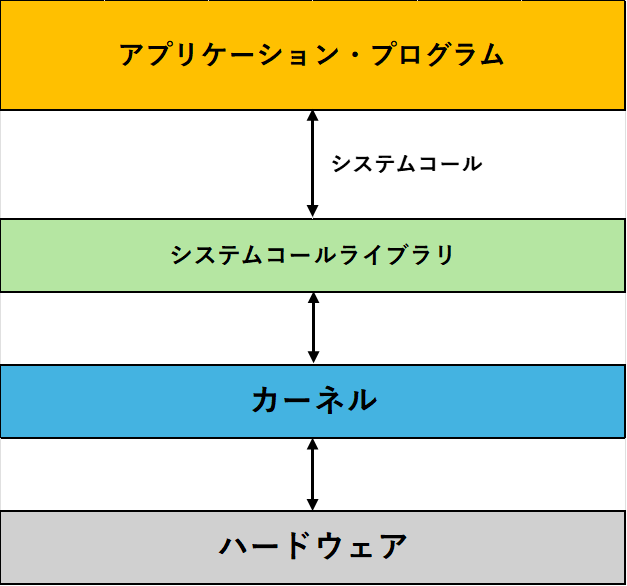
\includegraphics[width=80mm]{image/kernel-system.png}
    \caption{カーネル・プログラム・ハードウェアの連携}
    \label{fig:kernel}
\end{figure}

\subsection{まとめ}
\begin{itemize}
    \item OSはハードウェア資源やファイル・プロセスの管理を行っている
    \item カーネルはOSの中核的な役割を果たしており,ハードウェアの資源を利用した機能をソフトウェアに提供する
    \item 外部入力装置の処理などをプロセス管理と合わせて行っている
\end{itemize}



\section{ディレクトリとその構造}
OSはユーザーやプログラム・アプリケーションがファイルを利用しやすいように
フォルダやディレクトリという入れ物,あるいは階層と比喩される構造により管理している.
呼び方はOSなどで異なるが,基本的には「\textbf{木構造}」あるいは「\textbf{階層構造}」
と呼ばれる構造になっている.

\subsection{木構造}
木構造は節と枝という概念により構成され,最上位の「根」という節から枝が分かれ,その先に節が付いた木ような構造である.
また,末端の節を「\textbf{葉}」,枝により繋がっている節について,枝の派生元の節を「\textbf{親}」,派生先のものを「\textbf{子}」と呼ぶ.

例として岡山大学工学部の組織関係を以下の木構造で表す.
\begin{figure}[H]
    \centering
    \begin{forest}
        [\doublebox{岡山大学}
            [\Ovalbox{工学部}
                [\fbox{機械システム系}]
                [\fbox{情報・電気・DS系}]
                [\fbox{化学・生命系}]
                [\fbox{環境社会基盤系}]
            ]
        ]
    \end{forest}
    \caption*{岡山大学工学部の組織関係の木構造}
    \label{fig:okadai-tree}
\end{figure}

まず,上下関係において最上位の階層である「岡山大学」という枠組みがこの構造においての「根」にあたる.
そしてその一つ下の階層である「工学部」という枠組みは「岡山大学」を親にもつ「節」である.
更にその下には「工学部」を親に持つ4つの系が枝分かれして「葉」(末端の節)となっている.
このように階層や枠組みの上下関係とその繋がり・関係性が節とそれらから分かれる枝により表現される.

上記のような表現とは別に,コンピュータ内におけるディレクトリ構造を表す際によく使われる
「ディレクトリツリー構造」を用いて同様の関係をより細かく示す.
\DTsetlength{1.5em}{3em}{0.1em}{1pt}{4pt}
\begin{figure}[H]
    \dirtree{%
        .1 \doublebox{岡山大学}.
        .2 \Ovalbox{工学部}.
        .3 \fbox{機械システム系}.
        .4 機械工学.
        .4 ロボティクス・知能システム.
        .3 \fbox{情報・電気・数理データサイエンス系}.
        .4 情報工学.
        .4 ネットワーク工学.
        .4 エネルギー・エレクトロ二クス.
        .4 数理・データサイエンス.
        .3 \fbox{化学・生命系}.
        .4 応用化学.
        .4 生命工学.
        .3 \fbox{環境社会基盤系}.
        .4 都市環境創成.
        .4 環境マネジメント.
    }
\end{figure}

表現は違うものの,木構造と同じ上下関係を示した構造である.

\subsection{ディレクトリ構造}
ディレクトリ構造(あるいはファイルシステム)は前節の工学部組織と同様に
ディレクトリやファイルを節として,親子関係がある木構造が形成されている.

例としてWindowsのファイルシステムを見てみよう(以下,「フォルダ」は「ディレクトリ」と同じ意味です).まず,Windowsでフォルダやファイルの管理を行う「エクスプローラ」というアプリケーションを
開くと左側に「デスクトップ」や「ダウンロード」などのフォルダが置かれている部分があります.これの下側に移動すると「PC」と表示された項目があるので
クリックしてみましょう.すると以下の図\ref{fig:win_CDrive}ような表示が出ます.

この「OS (C:)」というのが「Cドライブ」と呼ばれる,Windowsのファイルシステムにおける「根」にあたる階層(フォルダ)で,これより下の階層にあらゆるフォルダやファイルが全て格納されています.
コンピュータのストレージや記憶域そのものとも比喩できます.

\begin{figure}[H]
    \centering
    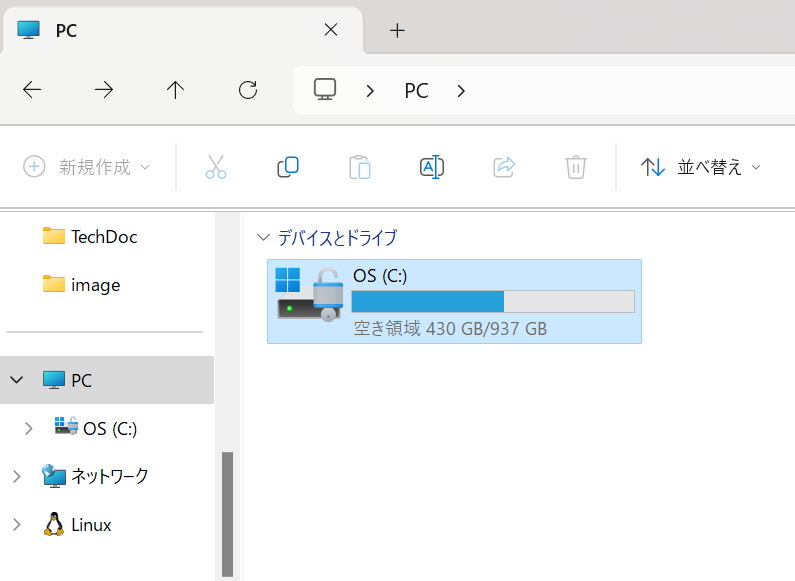
\includegraphics[width=120mm]{image/win_CDrive_img.png}
    \caption{WindowsのCドライブ}
    \label{fig:win_CDrive}
\end{figure}

このCドライブをクリックして内容を見てみると,中に「Microsoft」「Program Files」「software」の
様にコンピュータのシステムやソフトウェアに関するフォルダが格納されていて,
同じように適当にフォルダを開いてみると,またその中にフォルダがあるという感じになっていると思います.

\begin{figure}[H]
    \centering
    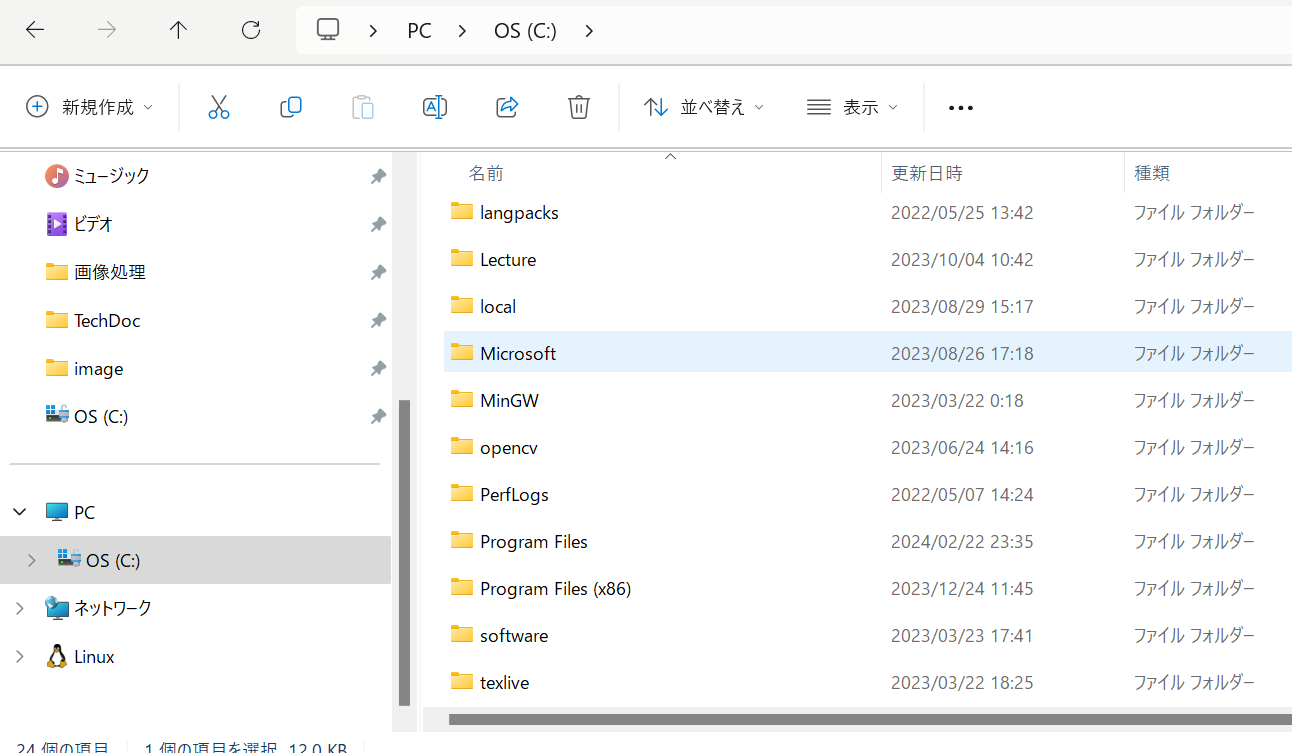
\includegraphics[width=120mm]{image/win_folders.png}
    \caption{Cドライブ直下のフォルダ}
    \label{fig:win_folders}
\end{figure}

この操作は木構造の上で根であるCドライブから枝分かれしている節,つまり子であるフォルダに移動していると表現できます.
先ほどの図をもとに簡単に木構造を書いてみると以下のようになります.

\begin{minipage}{7cm}
    %\DTsetlength{1.5em}{3em}{0.1em}{1pt}{4pt}
        \dirtree{%
        .1 \fbox{C:$\backslash$}.
        .2 \fbox{Microsoft}.
        .2 \fbox{Program Files}.
        .2 \fbox{software}.
        .2 \fbox{user}.
        .3 \fbox{user1}.
        .3 \fbox{user2}.
        }
\end{minipage}
\begin{minipage}{8cm}
    \begin{forest}
        [\fbox{C:$\backslash$}
            [\fbox{Microsoft}]
            [\fbox{Program Files}]
            [\fbox{software}]
        ]
    \end{forest}
\end{minipage}
\\

基本的にフォルダAの中にあるフォルダBがあるとすれば,BがAの中(または下)にあるという関係性になります.
また,エクスプローラー上のフォルダの左側にある\verb|>|のマークをクリックすれば,上図左の様にそのフォルダの中身が展開されます.

\subsection{パス}
本節ではプログラム開発において重要な「パス (Path)」についての解説を行います.第\ref{part:Linux}部以降でも頻出するので
是非覚えてください.

「パス」とはコンピュータ上におけるディレクトリやファイルの所在を示す概念のことで,現実のものに例えると「住所」にあたる.
パスには「\textbf{絶対パス}」と「\textbf{相対パス}」が存在します.
それぞれ例を交えつつ解説します.

\subsubsection{絶対パス}
絶対パスとは,ファイルシステムの一番上の階層(木構造でいう根)のディレクトリ(ルートディレクトリ)
から目的のファイルやディレクトリへ辿ったパスのことです.少々分かりにくいので住所を例に考えてみましょう.

ネットショッピングで商品を注文するときには,必ず家の住所が必要ですよね.その時指定する住所って基本的に
都道府県・市や区・町や群・番地というように大きい範囲から順に場所を絞っていき,その範囲の中からさらに特定の範囲を指定するという感じになります.
もしかしたら国から始まる場合もあるかもしれません.このような住所の指定の仕方は,たとえ配達側がその町を知らなかったとしても日本にいれば必ず分かる形式になっています.
つまり「日本国内であれば必ず特定できる絶対的な住所」というわけです.コンピュータにおける絶対パスはこの例において
\begin{itemize}
    \item 家 $\rightarrow$ ファイル・ディレクトリ
    \item 都道府県・市区町村などの区分 $\rightarrow$ 目的のファイル・ディレクトリが格納されているディレクトリ(木構造でいう親)
\end{itemize}

に置き換えたものになります.住所を言うときに「岡山県の,岡山市の,北区の,津島中一丁目の,1-1」
というように目的のファイルは「ルートディレクトリの中の,AAディレクトリの中の,BBディレクトリの中」であるといった感じです.

例として以下のLinuxのディレクトリ構造における\verb|File.h|というファイルの絶対パスを考えます.
パスは基本的に,辿っていくディレクトリをスラッシュ(\verb|/|)またはバックスラッシュ(\verb|\|)によって区切って順に並べていき,
最後に目的のファイルまたはディレクトリが来るように表記されます.
つまり,区切りの前後のディレクトリまたはファイルには親子関係があるということです.
下の図で四角形で囲んでいるのはディレクトリです.\\
(Linuxにおける一番上のディレクトリは「/」ルートディレクトリという)

\begin{figure}[H]
    \centering
    \begin{forest}
        [\Ovalbox{/}
            [\ovalbox{dev}
                [\ovalbox{input}
                    [event0]
                    [js0]
                ]
                [\ovalbox{bus}]
            ]
            [\ovalbox{opt}]
            [\ovalbox{proc}]
            [\ovalbox{home}
                [\ovalbox{{\color{blue}program}}
                    [config]
                    [\ovalbox{include}
                        [File.h]
                        [mylib.h]
                    ]
                    [\ovalbox{src}
                        [func.c]
                        [main.c]
                    ]
                ]
            ]
        ]
    \end{forest}
    \caption{例:絶対パス}
    \label{fig:abs-path-example}
\end{figure}

この時の\verb|File.h|の絶対パスは
\begin{center}
    \ovalbox{\large{\textbf{/home/program/include/File.h}}}
\end{center}
と表せます.ここで,Linuxではパスの表記においてルートディレクトリとその直下のディレクトリとの間にはスラッシュを挟まず,
ルートディレクトリを示すスラッシュの後にすぐ次のディレクトリ名を記述します.この部分だけ特別なので注意してください.

\subsubsection{相対パス}
相対パスとは,目的のファイルやディレクトリを自身がいるディレクトリである「カレントディレクトリ」を基点として
そこから辿ったときのパスのことである.基本的に目的となるファイル・ディレクトリがカレントディレクトリ
以下の階層に存在するときに使用される.

例として図\ref{fig:abs-path-example}で青色で示している\verb|program|ディレクトリをカレントディレクトリとしましょう.
このとき,直下にある\verb|config|というファイルの相対パスは
\begin{center}
    \fbox{\large{\textbf{config}}}
\end{center}
とそのまま表せます.自身のディレクトリに存在し,他にディレクトリを経由しなくても参照できるので当然です.相対パスにはカレントディレクトリを含まないことに注意です.
次に,\verb|myllib.h|と\verb|func.c|はそれぞれ
\begin{center}
    \ovalbox{\large{\textbf{include/mylib.h}}} \ \ \ovalbox{\large{\textbf{src/func.c}}}
\end{center}
と表せます.絶対パスと同様に経由したディレクトリを順に,最後に対象が来るように記します.

\subsection{まとめ}
\begin{itemize}
    \item ディレクトリ構造・ファイルシステムはどのOSでも基本的に木構造となっている
    \item ディレクトリ構造には根にあたる最上位の階層:ルートディレクトリが存在する
    \item パスとはディレクトリ構造において,特定のファイルやディレクトリの所在を示すものである
    \item パスには絶対パスと相対パスがあり,絶対パスはルートディレクトリから辿ったパス,相対パスはカレントディレクトリを基点としたパスである
\end{itemize}
このパスの概念は非常に大切なのでぜひ覚えてください!

\section{ターミナル・シェル}
ここでは様々なOSに標準で搭載されているターミナルとシェルについて解説します.
前章のパスと同様にプログラム開発はもちろん,特にLinux系のOSにおいて重要な要素です.

\subsection{ターミナル}
ターミナルとは,コンピュータやOSのシステムやアプリケーションの機能など
をユーザーが操作するためのコマンド操作が可能なCLI(コマンドラインインターフェース)を提供するアプリケーションのことを指す.
これに対する入力を処理しているのが後述するシェルである.

似たようなもので「コマンドプロンプト」という言葉があるが,ここでは一緒のものとして捉えてもらって構わない.
以下はWindows上で実行できるLinux環境「WSL2」のUbuntuのターミナルである.基本的にコマンド操作のみを行う.

\begin{figure}[H]
    \centering
    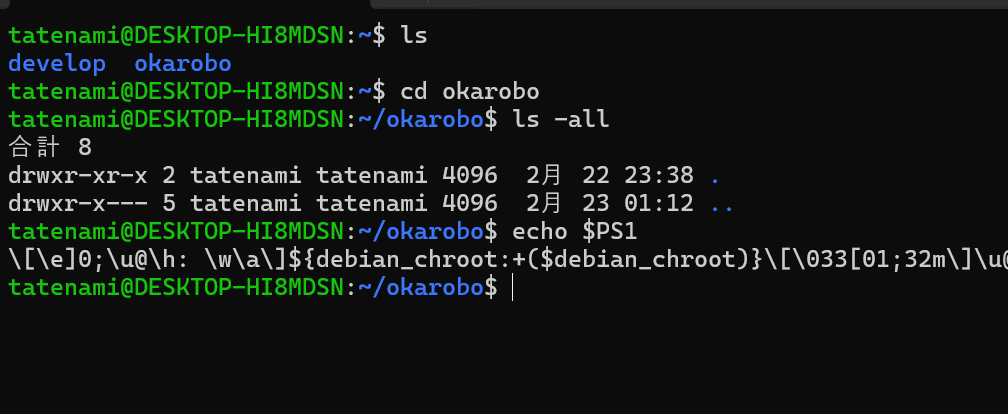
\includegraphics[width=150mm]{image/Terinal.png}
    \caption{Ubuntuのターミナル}
    \label{fig:Terminal}
\end{figure}

\subsection{シェル}
シェルとは,ユーザーとOSとの仲介を行うソフトウェアプログラムのことで,
ターミナルなどから入力されたコマンドの情報からOS(カーネル)へ命令や処理の伝達と
それに対する処理結果の表示などを行う.

シェルには様々な種類があり,代表的なものに
\begin{itemize}
    \item \textbf{sh}:Rourne Shell
    \item \textbf{bash}:Bourne-Again Shell
    \item \textbf{zsh}:Z Shell
    \item \textbf{fish}:Friendly interactive shell
\end{itemize}
などがある.特にbashはUNIX系・Linux系OSの標準シェルとして
広く利用されている.


\clearpage
\part{LinuxOSの基本とその操作} \label{part:Linux}
さて,事前知識の部分がかなり長くなってしまいましたが,ここからはいよいよ資料の本題でもあるLinuxについて
の解説を行います.大まかな流れとしては
\begin{enumerate}
    \item LinuxOSに関する歴史と,それにまつわる重要な要素
    \item Linuxにおけるコマンド操作
    \item シェルの操作とプログラム
\end{enumerate}
という感じで進めていきます.

\section{LinuxOSとは?}
本章では

\subsection{UNIX}

\subsection{LinuxOS}

\subsection{Linuxディストリビューション}

\subsection{GNU}

\subsection{その他の重要なシステム・要素}



\section{コマンドの操作}
本章では実際にLinuxでよく使用するコマンド操作について解説します.資料の概要にも示したように
解説で使用しているOSは\textbf{Ubuntu} (ver: 22.04)ですが,LinuxあるいはUnix系であればどのOSであっても
基本的に同じことができるので,この資料と同様の操作をする際に別の環境を使用していても問題ありません.OSによっては使えなかったり挙動が
異なる事柄に関しては,都度そのことを記します.

\subsection{そもそもコマンドとは?} \label{sec:command_example}
先程からLinuxと共に「コマンド」という言葉を出していますが,コマンドとは何なのでしょうか?
簡単にいうと,コマンドは「CLI上でのコンピュータに対する命令」のことです.
Ubuntuでのターミナルを示した図\ref{fig:Terminal}中での
\begin{center}
    「\texttt{ls} 」 \ 「\texttt{cd okarobo} 」
\end{center}
などがこれにあたります.
CLIでコマンドを打ち込むと
それに応じた処理をコンピュータが行ってくれます.これだけ聞くと「GUI上でアプリとかを使ってすればいいのではないか」
と思うかもしれません.当然コマンドで行える操作を同じ様にアプリケーションで実行できることは多いです.
ですが,プログラム開発で頻繁に行う\textbf{ファイルやディレクトリの操作}や\textbf{ネットワーク通信処理},\textbf{ソフトウェアやツールの管理}
などの重要な操作はコマンドの方が効率よく,かつ容易に実行することができたり,特有の機能を持っていることがあります.
そのため,Linuxを用いた開発においてはコマンドを覚えて使えることがとても大切なのです.


\subsection{基本的な使用・操作方法}
コマンド操作を行うためにはターミナルを立ち上げる必要があります.これには主に
\begin{itemize}
    \item GUI上でのアプリケーションの実行
    \item キーボードのショートカットによる起動
\end{itemize}
の2種類があります.

\subsubsection*{・\underline{アプリケーションを使った実行}}
Ubuntuではデスクトップ画面のタスクバー,あるいはアプリケーションの一覧に「端末」という名前のアイコンがあると思います.
これをクリックすれば図\ref{fig:Terminal_Ubuntu}の様なターミナルが立ち上がります.基本的に,黒い背景に「\textgreater」の様な矢印マークがついているものがターミナルになります.

また,図\ref{fig:Ubuntu_Menu}の様にデスクトップ画面上でマウスの右クリックにより出てくるメニューの「端末で開く」から起動する方法もあります.

\begin{figure}[H]
    \centering
\begin{minipage}[h]{0.45\linewidth}
    \centering
    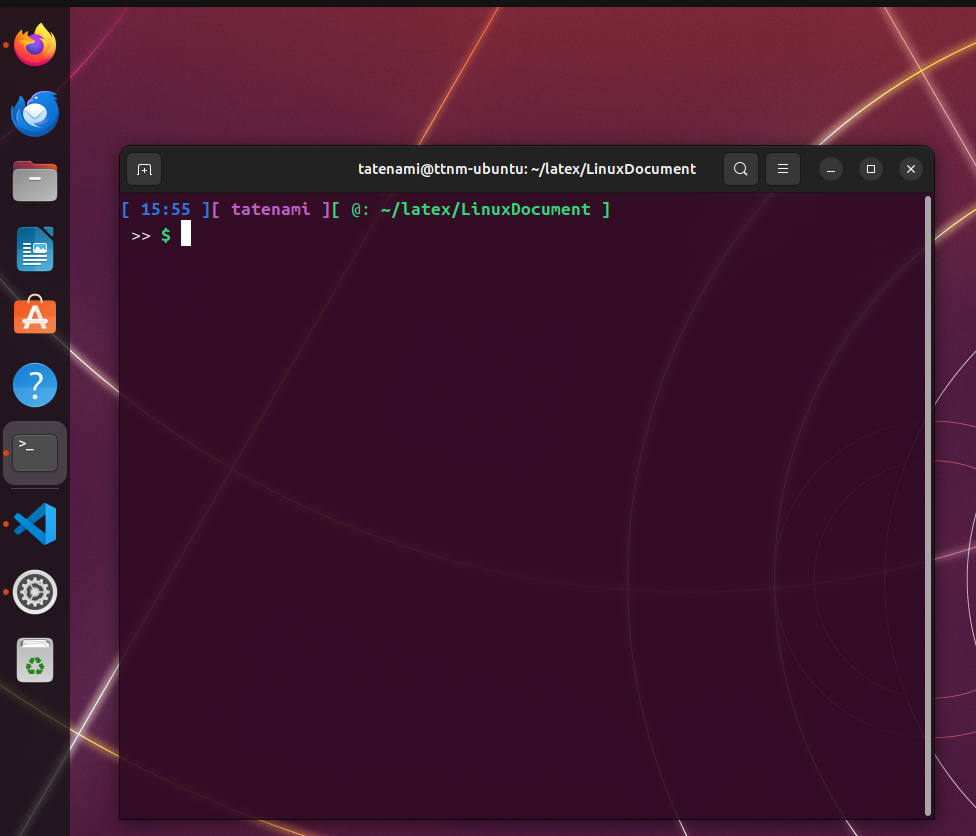
\includegraphics[width=60mm]{image/Terminal_ubuntu.png}
    \caption{Ubuntuのターミナル}
    \label{fig:Terminal_Ubuntu}
\end{minipage}
\hspace{10mm}
\begin{minipage}[h]{0.45\linewidth}
    \centering
    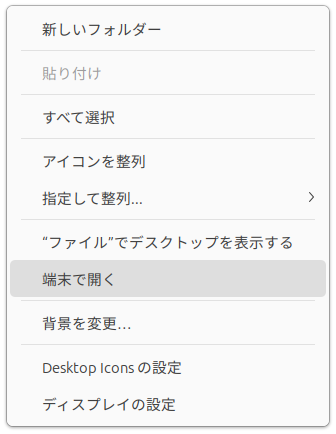
\includegraphics[width=50mm]{image/Ubuntu_Menu.png}
    \caption{右クリックで表示されるメニュー}
    \label{fig:Ubuntu_Menu}
\end{minipage}
\end{figure}

\subsubsection*{・\underline{キーボードのショートカットによる起動}}
Ubuntuではデフォルトの設定で,キーボードから
\begin{center}
    \ovalbox{\Large{ Ctrl + Alt + T }}
\end{center}
を押すことでショートカット機能によりターミナルを起動できます.わざわざマウスを使ってアプリを選択するよりも簡単なのでこちらの方法がおすすめです.
また,これによりターミナルの多重起動も素早くできるのも開発において大きな利点です.

\paragraph*{注意点}
以降の節ではコマンド操作の例を図や文章として説明しますが,その際登場するコマンド文字列中の文字間
の隙間はすべて「\textbf{半角スペース} 」です.第\ref{sec:command_example}節の「\texttt{cd okarobo} 」の「cd 」と「okarobo 」
の間も半角スペースです.これはコマンド入力において半角スペースがコマンドやオプションなどの複数のパラメータを識別する
「\textbf{区切り}」の役割を果たしているからです.本来ひと続きの文字列の途中に誤って半角スペースを入れてしまうと,その文字列が正しく認識されなかったり,
エラーを吐かれたりするので気を付けましょう.この仕様はLinuxに限らず基本的にどのOSのターミナルでも同じです.

\subsection{コマンドの基本的な書式・構文}
コマンドはアルファベットの文字列であり,コマンドとして認識される文字列を正しく入力すれば
そのコマンドの処理が実行されます.ターミナルには「プロンプト」と呼ばれる,ユーザーやカレントディレクトリなどの情報が記された文字列
があり,基本的にこの後ろ側でキーボードが入力待機の状態となっているので,ここにコマンドを入力します.

下に示したターミナルを例にコマンド入力について簡単に説明します.
\begin{itemize}
    \item ドルマークまでの文字列は「プロンプト」です.ターミナルの入力の際に
    勝手に現れます.シェルによってデザインが違ったりします.
    \item プロンプト内の青色の文字列はカレントディレクトリのパスです.
    これは基本的にターミナル起動時は「\textbf{\textasciitilde}」(チルダ)で表される,ユーザーのホームディレクトリが仮の頂点ディレクトリとなって表示されます.
    従ってここに記されるパスは,ホームディレクトリ以下の階層で作業する場合にはこのホームディレクトリを基点とした相対パスとなりますが,
    もしホームディレクトリより上のルートディレクトリなどに移動した場合は絶対パスなどになります.
    \item プロンプト以降に示した文字列が「コマンド入力」となります.コマンド入力は黄色の文字が「コマンド」,
    下線が記され,ハイフンついた文字からはじまるがコマンドの「オプション」,それ以外の文字列は,コマンドまたはそのオプションの引数
    となります.また,入力する順番が決まっている引数はオプションと合わせて下線を引いている場合があります.(例:\verb|gcc|の\verb|-o|オプションなど)
\end{itemize}


\begin{figure}[H]
    \begin{terminal}{ターミナル上でのコマンドの例}
        \termtext{\textasciitilde/dir}{\cmd{command} \underline{-x} arg}
    \end{terminal}
    \caption*{コマンド入力を行うターミナルの例}
\end{figure}

また,ディレクトリ操作やパスにあまり関係が無いコマンドの例では以下の様にパスを示さないプロンプト
の表記をします.

\begin{figure}[H]
    \begin{terminal}{簡単なプロンプト表記}
        \termtext{}{\cmd{command} \underline{-x} arg}
    \end{terminal}
    \caption*{簡易表記のプロンプトを用いたターミナルの例}
\end{figure}

\subsection{コマンドのオプション}
前節で出てきたコマンドの「オプション」とは,
\textbf{コマンドの動作や出力などの機能を指定・カスタマイズすることができる入力}のことを指します.
コマンドごとにオプションが用意されており,それらは\verb|man|コマンドなどで確認することができます(第\ref{sec:cmd_man}項).
基本的には前節で示した様に,コマンドの後に入力し,
\begin{center}
    「ハイフン」$+$ 「アルファベット」
\end{center}
という構文になっています.
他にもハイフンが二つ連続で並ぶものもあったりするので,実際にコマンドとそのオプションを頻繁に使用する際は調べると良いでしょう.

オプションは一回のコマンド操作で複数指定することができます.
例として\verb|command|というコマンドに「\verb|-a|」,「\verb|-b|」
の二つのオプションを指定するには以下の様に
\begin{itemize}
    \item 別々に入力する方法
    \item 連結させて入力する方法
\end{itemize}
の二つの方法があります.

\begin{figure}[H]
    \begin{terminal}{別々に入力}
        \termtext{}{\cmd{command} \underline{-a} \underline{-b}}
    \end{terminal}
\end{figure}

\begin{figure}[H]
    \begin{terminal}{連結させて一括で指定}
        \termtext{}{\cmd{command} \underline{-ab}}
    \end{terminal}
\end{figure}

\subsection{ファイル・ディレクトリ操作}
ファイルやディレクトリの操作によく使う基本的なコマンドを以下に示す.

\begin{table}[H]
    \centering
    \begin{tabular}{|c|c|}
        \hline
        コマンド & 機能 \\
        \hline
        \verb|pwd| & 現在のカレントディレクトリを表示する \\
        \hline
        \verb|ls| & ディレクトリ内の一覧を表示する \\
        \hline
        \verb|cd| & ディレクトリの移動 \\
        \hline        
    \end{tabular}
\end{table}

また,本章でコマンド操作の例で使用するディレクトリ構造について,ホームディレクトリ以下の階層は下記の様な構造になっているとする.
\begin{figure}[H]
    \centering
    \begin{forest}
        [\fbox{home}
            [\fbox{user1}
                [\fbox{test}
                    [CMakelists.txt]
                    [\fbox{include}]
                    [\fbox{src}]
                ]
                [\fbox{okarobo}
                    [\fbox{ros2\_ws}]
                    [memo.txt]
                ]
            ]
        ]
    \end{forest}
    \caption{本節の例で使用するディレクトリ構造}
    \label{fig:file_dir_exam_tree}
\end{figure}

\subsubsection{\texttt{pwd}コマンド}
\verb|pwd|は「Print Working Directory」の略であり,
実行すると現在のカレントディレクトリの絶対パスを表示します.

例として,カレントディレクトリがユーザーのホームディレクトリ(\verb|user1|)であるとする.
実行すると以下の様に表示される.

\begin{figure}[H]
    \begin{terminal}{pwdコマンド}
        \termtext{\textasciitilde}{\cmd{pwd}} \\
        \texttt{/home/user1}
    \end{terminal}
\end{figure}


\subsubsection{\texttt{ls}コマンド}
\verb|ls|コマンドは,引数で指定されたパスのディレクトリ内の一覧(ファイルとディレクトリ)
を表示する.基本的な使い方は以下の様になる.

\begin{figure}[H]
    \begin{terminal}{lsの基本構文}
        \termtext{}{\cmd{ls} \underline{options} directory\_path}
    \end{terminal}
\end{figure}

ここで,引数として指定するディレクトリのパスは絶対パス・相対パスのどちらでも良い.
\underline{引数が無い場合はカレントディレクトリ内の一覧}を表示する.
以下,ホームディレクトリで引数無しで\verb|ls|コマンドを実行したときの例を示す.

\begin{figure}[H]
    \begin{terminal}{引数無しでの実行}
        \termtext{\textasciitilde}{\cmd{ls}} \\
        \texttt{\textcolor{dircolor}{test okarobo}}
    \end{terminal}
\end{figure}

カレントディレクトリがホームディレクトリ(\verb|user1|)の時に,相対パスにより\verb|test|
ディレクトリ内の一覧を表示するには以下の様に入力する.

\begin{figure}[H]
    \begin{terminal}{引数に相対パスを指定して表示}
        \termtext{\textasciitilde}{\cmd{ls} test} \\
        \texttt{\textcolor{dircolor}{include src} CMakelists.txt}
    \end{terminal}
\end{figure}

\paragraph*{ \texttt{-a,-all}オプション}
\verb|ls|コマンドに\verb|-a|または\verb|-all|オプションを指定して
実行すると,通常は表示されない,先頭が「.」から始まる「隠しファイル」も含めて表示される.

\begin{figure}[H]
    \begin{terminal}{隠しファイルも表示}
        \termtext{\textasciitilde}{\cmd{ls} -a} \\
        \texttt{\textcolor{dircolor}{.} \ \ \ \ .bashrc \ \ \ \textcolor{dircolor}{test}} \\
        \texttt{\textcolor{dircolor}{..} \ \ \ .vimrc \ \ \ \ \textcolor{dircolor}{okarobo}} 
    \end{terminal}
\end{figure}

上記の例ではホームディレクトリで\verb|-a|オプションを指定して実行した例である.
実際にLinux上で表示されるものを多少省いている.
ここで,隠しファイルとして表示された「.」はカレントディレクトリを,「..」は一つ上のディレクトリを示すものである.

\subsubsection{\texttt{cd}コマンド}


\subsubsection{\texttt{man}コマンド} \label{sec:cmd_man}

\subsubsection{\texttt{sudo}コマンド}

\subsection{ソフトウェア・パッケージ管理:\texttt{apt}}

\clearpage
\part{応用編}

\section{make}

\end{document}